\section{Architektura překladače}

Průběh překladu řídí \texttt{main.c}. Lexikální analyzátor čte zdrojový program IFJ26 ze standardního vstupu a na vyžádání předává parseru jednotlivé tokeny. Parser z nich sestaví abstraktní syntaktický strom. Sémantická analýza tenhle strom zkontroluje a doplní do něj informace o typech. Při vyhledávání jmen a kontrole deklarací využívá tabulky symbolů.

Ověřený AST převezme modul \texttt{insidecodegene} a vytvoří z něj seznam instrukcí \texttt{ListOfInstr}. Seznam spravuje modul \texttt{ilist}. Každá instrukce v něm má určený druh a až tři operandy. Modul \texttt{codegen} seznam postupně projde a vypíše výsledný kód IFJcode26 na standardní výstup.

Při chybě se překlad ukončí s příslušným návratovým kódem. Diagnostika se vypisuje na standardní chybový výstup.

\begin{figure}[h]
  \centering
  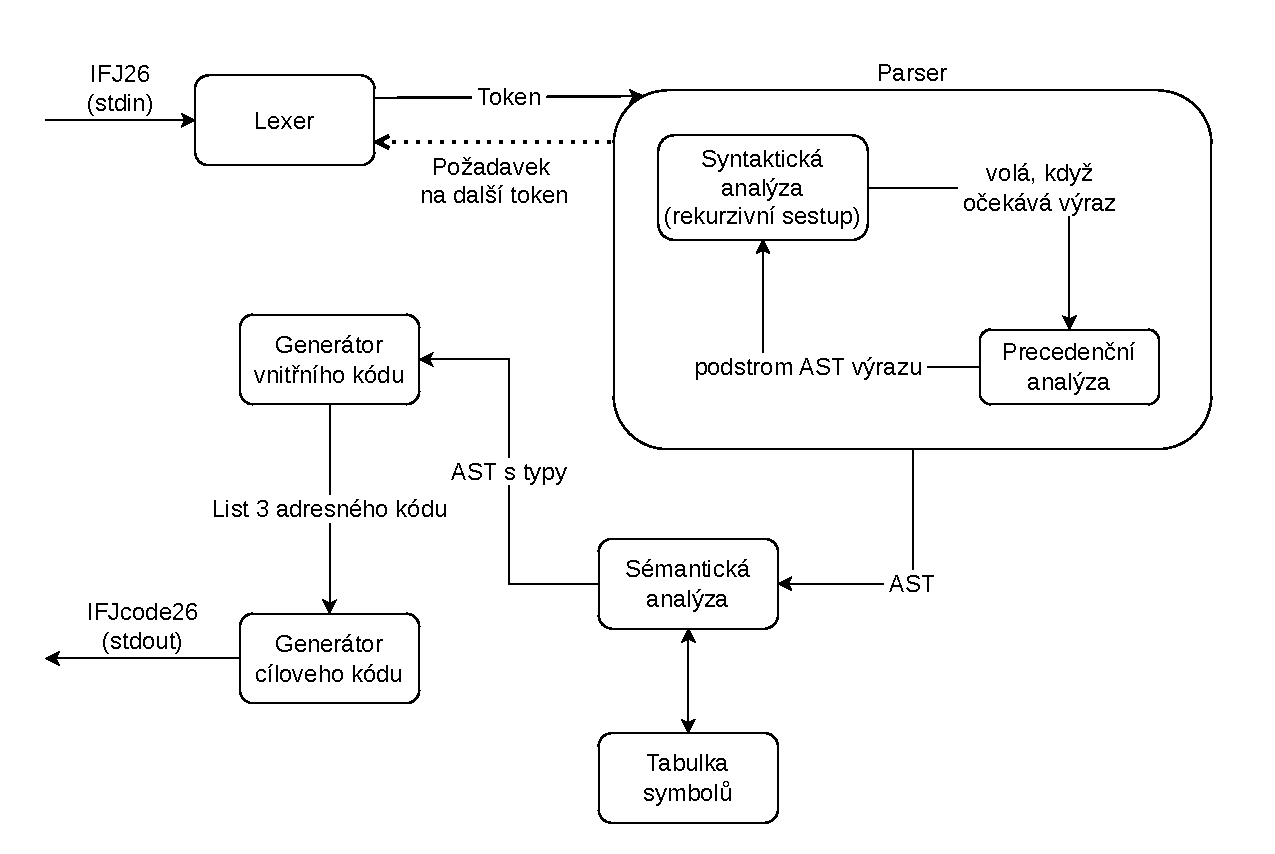
\includegraphics[width=\linewidth]{casti/blokove_schema.pdf}
  \caption{Blokové schéma architektury překladače}
  \label{fig:architektura}
\end{figure}